\newpage
\section{Trabalhos relacionados}
\label{sec:related}

Apresentaremos nesta seção, uma revisão de trabalhos relacionados
com a NetFPGA. Destaca-se que desde 2006, quando o projeto ganhou
maior popularidade, já foram publicados mais de 226 artigos
acadêmicos envolvendo a NetFPGA como parte de pesquisa cientifica em
redes de computadores ou sistemas distribuídos, e existe uma extensa
listagem de mais de 40 projetos com código aberto, tanto nas versões
de NetFPGA 1G quanto nas versões mais recentes da NetFPGA 10G, CML e
SUME. Nesta breve revisão destacaremos as contribuições mais
importantes.

\subsection{Artigos Acadêmicos}

A plataforma NetFPGA teve sua origem em um curso de pós-graduação
CS344 de Stanford~\cite{4589059}, onde os alunos trabalhavam em um
projeto para criar um roteador tanto com componentes em
\textit{hardware} e em \textit{software} em oito semanas. Parte da
motivação deste curso, veio da experiencia na indústria de alguns
dos professores como Nick McKweon (um dos arquitetos do roteador
Cisco GSR 12000). Na indústria, destacava-se que os estagiários e
recém-contratados, ou entendiam bem de \textit{hardware} ou
entendiam bem de \textit{software}, mas não os dois ou sua
integração. Adicionalmente ao ensino, a construção de um sistema
aberto como a NetFPGA também propiciou um ambiente para pesquisa de
alta qualidade em redes~\cite{Naous:2008:NRR:1397718.1397720}.

Dentre os primeiros projetos, os alunos do curso contribuíram com
roteadores e comutadores de referência, bem como sistemas de
monitoração de \emph{buffers} e geradores de pacotes altamente
precisos~\cite{5290917}. Em 2008, auxiliado pela popularidade da
tecnologia OpenFlow, foi desenvolvido uma implementação de um
comutador OpenFlow em NetFPGA~\cite{Naous:2008:IOS:1477942.1477944}.
Esta foi uma das primeiras soluções de comutador OpenFlow flexíveis,
de alta velocidade e baratas para pesquisa em SDN. E posteriormente,
tornou a NetFPGA um elemento presente em ambientes de produção de
diversas plataformas de experimentação OpenFlow internacionais como
GENI, KOREN e o FIBRE~\cite{1649119}.

Os projetos de desenvolvimento foram ganhando mais sofisticação
dentro de vários \textit{Workshops} de Desenvolvimento específicos
em NetFPGA, tanto em Stanford quanto em Cambridge-UK, e em outras
partes do mundo.  Esses \textit{Workshops} popularizaram trabalhos
técnicos em várias áreas, que faziam uso da plataforma. Adicionando,
por exemplo, projetos em suporte a \textit{drivers} para Windows ou
a implementação de protótipo de envio de sinal de rádio GNURadio
empacotado em pacotes IP~\cite{airnetfpga}.

Outros trabalhos oriundos dos \textit{Workshops} concentram as
publicações de trabalhos relacionados nos anos de 2009 e 2010. A
partir de 2011, a quantidade de trabalhos que usa ou avança o
progresso da NetFPGA aumenta consideravelmente, diversificando sua
atuação em diversas publicações especializadas em redes ou FPGAs em
congressos da ACM e IEEE, e portanto não mais restrito aos
\textit{Workshops}. Um pequeno resumo de alguns desses projetos
segue, ordenados cronologicamente:

\begin{itemize}

\item \textit{Fast Reroute and Multipath}~\cite{multipath}: trata-se
de um projeto onde a partir do roteador de referência foi adicionado
a possibilidade de recuperação de rotas por \emph{hardware}, em caso
de falha. E uma implementação do protocolo ECMP (\emph{Equal Cost
Multipath}) para realizar o balanceamento de carga de fluxos entre
as interfaces da NetFPGA.

\item \textit{NetThreads -- Programming NetFPGA with Threaded
Software}~\cite{6645624}: A ideia consiste na implementação de uma
arquitetura soft-core baseada em NetFPGA multiprocessada e
\emph{multithreaded}, para que aplicações de rede que têm
paralelismo inerente possam se beneficiar e acelerar aplicações
paralelas, com melhoria no compartilhamento dos dados e na
sincronização no nível físico.

\item \textit{DFA-based Regular Expression Matching}~\cite{dfa}:
Esse projeto trata de capturar através de regras do aplicativo
\textit{Snort} e usando expressões regulares transformadas em
autômatos determinísticos finitos (DFA) em \textit{hardware}. Desse
modo, determinados fluxos são capturados baseados em classificação
de cabeçalhos de pacotes. Os estados são manipulados na memória da
placa e também fora da mesma e existe um rastreamento da transição
de estados no chip para verificar se determinado pacote casa com uma
regra complexa.

\item \textit{OpenPipes -- Prototyping High-speed Networking
Systems}~\cite{openpipes}: Trata-se de uma plataforma de criação de
``sistemas distribuídos'' em \textit{hardware}, onde cada componente
pode ficar em um computador separado, interligado em rede. Esses
componentes se comportam como tubos (\textit{pipes}), tornando a
criação modular e simples, de sistemas baseados em \textit{hardware}
escaláveis. Na demonstração, os autores usam módulos de
processamento de vídeo embarcados na placa, como suavização de
imagem, conversão para tons de cinza e inversão de cores, e
separados em diferentes máquinas em rede, onde a execução
distribuída é feita com a ajuda da NetFPGA integrando os dados.

\item \textit{PortLand -- A Scalable Fault-Tolerant Layer 2 Data
Center Network
Fabric}~\cite{NiranjanMysore:2009:PSF:1592568.1592575}: Este
trabalho apresenta a concepção de uma rede de centro de
processamento de dados totalmente baseada em camada de enlace, com
tolerância a falhas e alto desempenho. Isso é obtido pelo reuso do
endereçamento MAC de maneira a permitir a migração de máquinas
virtuais intra-rack e inter-rack, e a manutenção de sua
conectividade IP. A avaliação do projeto, em alta velocidade, contou
com um conjunto de cerca de 40 NetFPGAs. Esse foi um dos primeiros
trabalhos a usarem a NetFPGA como apoio à validação experimental em
pesquisa em redes de alta velocidade.

\item \textit{BCube: A High Performance, Server-centric Network
Architecture for Modular Data
Centers}~\cite{Guo:2009:BHP:1592568.1592577}: Outro artigo na mesma
linha do Portland, focado em uma nova arquitetura de rede para
centros de processamento de dados. A ideia é um tipo de rede
centrada em interligação de servidores, sem apresentar equipamentos
de rede como comutadores ou roteadores. Os servidores agem como
encaminhadores de tráfego, além de pontos finais de comunicação.
Outras características importantes são tolerância a falhas e
balanceamento de carga. Destaca-se que a implementação da prova de
conceito foi toda feita em NetFPGA.

\item \textit{Using NetFPGA to Offload Linux Netfilter
Firewall}~\cite{netfilter}: O \emph{framework} Netfilter está
localizado na camada IP do Linux e é caracterizado por uma série de
ganchos (pontos de entrada) que permitem interceptar e manipular
pacotes que atravessam a camada IP. Normalmente, ferramentas como o
\ssf{iptables} permitem a comunicação direta com o Netfilter por
meio de soquetes Netlink, de modo a realizar chamadas de sistema nos
pontos dentro do \emph{kernel} e manipular ou descartar pacotes. O
projeto modifica o \ssf{iptables} e descarrega algumas regras
Netfilter direto para o \emph{hardware} por meio da NetFPGA,
liberando a CPU para outras atividades.

\item \textit{A Randomized Scheme for IP Lookup at Wire Speed on
NetFPGA}~\cite{5502019}: Os tempos de busca em uma tabela de
encaminhamento (chamados de \textit{lookups}) precisam ser em geral
muito baixos, embora o tamanho das tabelas na Internet só cresça.
Nesse sentido, os autores deste trabalho apresentam um novo esquema
de busca de endereços usando a NetFPGA, que faz uso de buscas em
paralelo feitas com funções de \textit{hash} perfeitas. Essas
funções trabalham com uma estrutura de dados de rápido acesso e
bastante compactas chamadas de \textit{Blooming Trees}.

\item \textit{BORPH: An Operating System for the NetFPGA
Platform}~\cite{borph}: O artigo BORPH apresenta o conceito de um
sistema operacional projetado para trabalhar com computadores
reconfiguráveis baseados em FPGA. A prova de conceito é feita por um
conjunto de extensões do Linux. Dado a facilidade de reconfiguração
pelo barramento PCI que a NetFPGA habilita, o sistema foca em prover
abstrações UNIX como arquivos, de modo a ter acesso direto a
recursos de registradores e processamento da NetFPGA bem como
reconfigurar partes do \emph{hardware} sob demanda.

\item \textit{The Click2NetFPGA Toolchain}~\cite{180848}: Nesse
trabalho, a ideia é facilitar a aceleração promovida pela NetFPGA na
área de aplicações em rede, através do uso de um sintetizador de
alto nível. Em resumo, a partir de uma descrição de um roteador com
linguagem de domínio e componentes básicos em C++ usados no
\textit{Click Modular Router}. O artigo se propõe a transformar
automaticamente código existente dentro desse domínio específico em
um projeto de \textit{hardware} funcional. A cadeia de ferramentas
faz uso de LLVM, como linguagem de abstração intermediária, depois
uma optimização usando uma técnica chamada AHIR que permite, a
partir de uma estrutura bem definida LLVM, produzir o código VHDL
para a NetFPGA.

\end{itemize}

Com essa revisão de trabalhos relacionados podemos verificar a ampla
cobertura e exuberante quantidade de desenvolvimento que a
plataforma NetFPGA tem atraído. No que segue nesta seção, daremos
destaque em maior profundidade a dois projetos de alto impacto para
a realização de pesquisas em redes: a implementação do comutador
OpenFlow na NetFPGA e o \emph{Software} Testador de Redes OSNT, que
permite geração de tráfego para testes de desempenho de alta
precisão.

\subsection{Implementação de OpenFlow na NetFPGA}

Nesta seção, descreveremos a implementação do OpenFlow em uma placa
NetFPGA~\cite{Naous:2008:IOS:1477942.1477944}. A princípio é preciso
observar que boa parte da complexidade do comutador OpenFlow é
oriunda de outros elementos NetFPGA de referência como partes da
placa de rede de quatro portas, comutador e roteador IPv4. A
implementação possui duas partes relevantes: o \emph{software} de
gerenciamento, lado que trata as mensagens do protocolo OpenFlow
1.0, e a aceleração da tabela de fluxos (\textit{flow table}) em
\emph{hardware}.

O \emph{software} de gerenciamento do comutador OpenFlow é baseado
na implementação de referência de comutadores OpenFlow de Stanford.
Trata-se de um \emph{software} aberto para Linux que implementa todo
o comportamento de um comutador OpenFlow. Este software de
referência pode ser dividido em duas seções: o programa que executa
em espaço de usuário e o módulo do \emph{kernel}.

O processo que executa em espaço de usuário se comunica por soquete
com o controlador OpenFlow usando SSL para criptografar a
comunicação.  O processo coordena o envio das mensagens do comutador
para o controlador e vice-versa, tratando chegadas de novos fluxos
ou atualizações do estado dos enlaces do comutador. As mensagens de
controle permitem adicionar ou remover entradas da tabela de fluxos
e são implementadas através de chamadas de sistema \ssf{ioctl} entre
o programa que executa em espaço de usuário e o módulo do
\emph{kernel}.

O módulo do \emph{kernel} é responsável por manter as tabelas de fluxo,
processar pacotes, encaminhar, reescrever cabeçalhos e atualizar
estatísticas.  Por definição, o módulo do \emph{kernel} do comutador
OpenFlow de referência cria a tabela de fluxo em \emph{software}, e vai
testando as cadeias de regras por um casamento sequencialmente. A
prioridade é dada para a primeira regra que casar dentro da cadeia.

Ainda no módulo do \emph{kernel} é possível estender a tabela de
fluxos para fazer uso de processamento em \textit{hardware} na
NetFPGA.  Os pacotes que chegam na NetFPGA fazem acesso rápido as
entradas da tabela de fluxo armazenadas na NetFPGA e encaminha os
pacotes com casamento na mesma taxa dos enlaces (por exemplo,
1\,Gbps por porta). Por sua vez, pacotes que não casem com regras de
fluxo existentes (por exemplo, fluxos novos) são enviados para o
módulo do \emph{kernel} do OpenFlow, onde serão tratados.  Pacotes
sem casamento podem chegar ao programa em espaço do usuário, que irá
gerar um evento \ssf{pkt\_in} e enviá-lo ao controlador.

\begin{figure}[h]
\centering
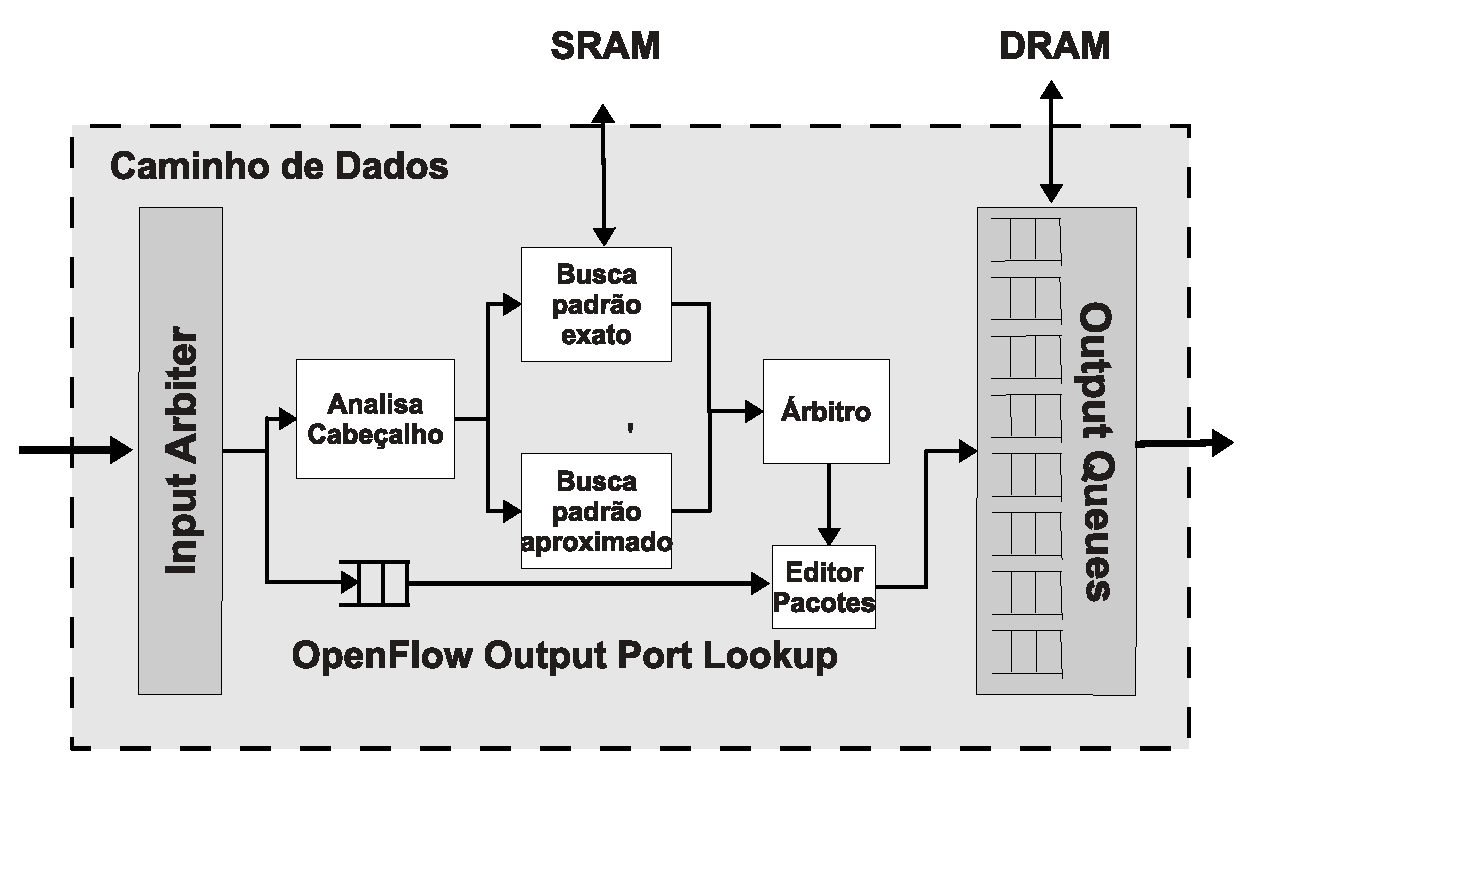
\includegraphics[scale=0.4]{figures/netfpga-rev/nfopenflow.eps}
\caption{Componentes do comutador OpenFlow NetFPGA.}
\label{fig:nfopenflow}
\end{figure}

Ilustramos o módulo \ssf{output\_port\_lookup} do comutador OpenFlow
na \figstr~\ref{fig:nfopenflow}.  Primeiro ele concatena cerca de
dez campos num cabeçalho de fluxo (\emph{flow header}), e envia esse
cabeçalho para busca nas tabelas de roteamento. A busca é feita em
paralelo utilizando uma combinação de memórias ternárias (TCAMs) no
FPGA e memória SRAM para suportar tanto a possibilidade de
``coringas'' (prefixos) na TCAM quanto um grande número de entradas
exatas de fluxos na SRAM.

Essa busca de entradas exatas utiliza de uma função de \emph{hash}
do cabeçalho de fluxo para indexar a SRAM, reduzindo a necessidades
de memória e colisões. Após o casamento de uma regra, o módulo
possui uma fase de tomada de ações, através de um árbitro.  O
árbitro pode editar campos do pacote antes de encaminhá-lo para as
filas de saída. Essa fase de ações está associada à sequência dos
casamentos, com uma ação definida para cada regra com casamento.

\subsection{OSNT: Open Source Network Tester}

O segundo projeto que descreveremos em maior detalhe é a
implementação de um testador de rede usando a
NetFPGA-10G~\cite{shahbaz2013arch}. A solução é código aberto e de
alto desempenho operando a 10Gbps, custa para um pesquisador pouco
menos de 2 mil dólares, sendo que equipamento equivalente em
\textit{hardware} na indústria especializada custa 25 mil dólares. A
placa usa um FPGA mais recente e tem a habilidade de trabalhar com
múltiplos \textit{pipelines} de processamento. Entre esses,
destacamos somente o subsistema de geração de tráfego, na figura
\ref{fig:osnt1}. Existem outros subsistemas, por exemplo para
encapsulamento de pacotes para virtualização e de monitoração
passiva e precisa de tráfego.

\begin{figure}[h]
\centering
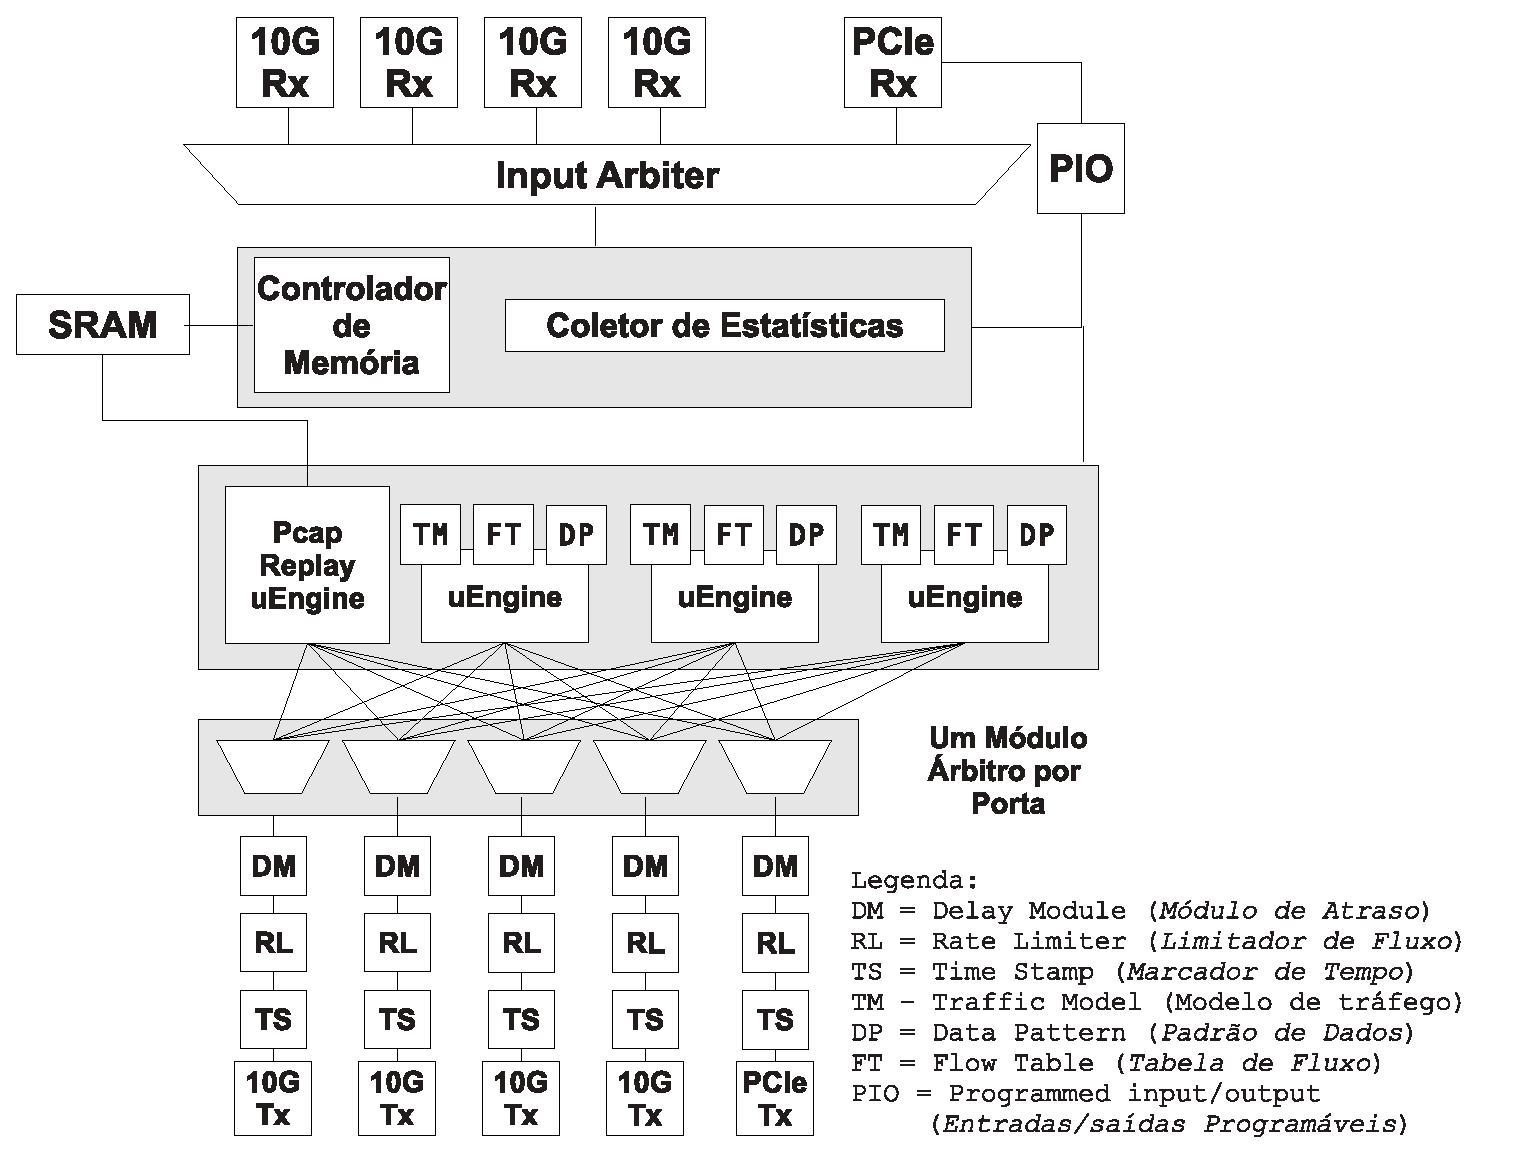
\includegraphics[scale=0.5]{figures/netfpga-rev/osnt1.eps}
\caption{\emph{Pipeline} de Geração de Tráfego da OSNT.}
\label{fig:osnt1}
\end{figure}

O \textit{pipeline} gerador de tráfego gera pacotes e analisa
estatísticas. O gerador de tráfego consiste de pequenos
\textit{micro-engines}, cada qual gera tráfego de acordo com um
modelo de tráfego (TM, \emph{traffic model}) configurado, uma lista
de valores para os cabeçalhos dos fluxos (FT) e certos padrões de
como gerar o tamanho do pacote, sua taxa e os atrasos entre pacotes
(DP).  Adicionalmente é possível gerar tráfego a partir de um
\textit{trace} \ssf{pcap} (via \ssf{tcpdump}). Após essa fase de
moldagem dos fluxos, existem cinco unidades funcionais para efetivar
a transmissão: o árbitro seleciona os pacotes e os encaminha quando
for o tempo correto de envio.  Depois, o módulo de atraso (DM)
controla o atraso, o módulo de limitação de taxa (RL) limita cada
fluxo (implementando algoritmo equivalente a um \emph{token
bucket}), o módulo de marcação de tempo (TS) computa quando o pacote
foi transmitido e por último o pacote é enviado.

\subsection{Futuro da NetFPGA: Projetos NetFPGA-10G, 10G-CML e 10G-SUME}

Redes de centros de processamento de dados vêm motivando a adoção de
sistemas de rede mais rápidos. As velocidades oferecidas pela
NetFPGA 1\,Gbps, embora interessantes do ponto de vista de ensino,
são bastante defasadas em termos de velocidade para pesquisa na área
de centros de processamento de dados.

Nesse sentido, o projeto NetFPGA, ao longo dos anos vem colocado a
disposição placas de 10\,Gbps, a mais recente com capacidade de I/O
de 100\,Gbps~\cite{6866035}. Dessa forma, o projeto fica atualizado
com relação a uma nova geração de dispositivos de alta velocidade.
Ou seja, permite testar novas ideias em escala compatível com
ambientes de centros de processamento de dados, em empresas como
Localweb, UOL, ou Facebook. A NetFPGA 1G era uma placa de baixo
custo projetada usando um FPGA Xilinx Virtex-II Pro 50. Por sua vez,
em 2010, foi lançada a placa NetFPGA 10G, que expandia a plataforma
original para trabalhar com transmissões até 40\,Gbps sendo 10\,Gbps
por interface, com interface PCIe Gen~1, e baseado no FPGA Xilinx
Virtex-5 FPGA.

Posteriormente, a placa 10G-CML desenvolvida pela empresa
especializada em segurança cibernética CML (\textit{Computer
Measurement Lab}), atualizou o FPGA para o Xilinx Kintex-7 325T, e o
I/O é baseado no adaptador PCIe x4 Gen~2, com alto desempenho. A
última linha de placa que surgiu em 2014 é a 10G-SUME~\cite{6866035}
conforme mostra a figura \ref{fig:sume}.

\begin{figure}[h]
\centering
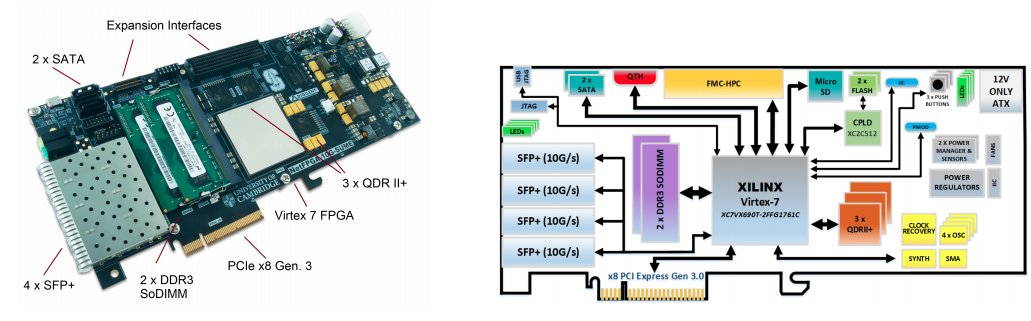
\includegraphics[scale=0.4]{figures/netfpga-rev/sume.png}
\caption{Foto e Arquitetura da Placa SUME.}
\label{fig:sume}
\end{figure}

A placa NetFPGA SUME é uma placa de custo mais elevado, porém o
preço é subsidiado para pesquisa acadêmica. Além disso ela possui
capacidade de I/O aumentada com operações de até 100\,Gbps através
do adaptador PCIe x8 Gen~3 e também incorpora um  FPGA mais poderoso
que é o Xilinx’s Virtex-7 690T. Para demonstrar as capacidades da
placa SUME, os pesquisadores utilizaram três placas para montar um
comutador OpenFlow com 12 interfaces de 10\,Gbps interligadas por um
\emph{backplane} não-blocante de 300\,Gbps.

Enfim, o futuro da NetFPGA parece bastante promissor em termos de
avanços na área de alto desempenho. O \textit{software} de todos os
projetos desenvolvido  está disponível no GitHub e é licenciado como
\emph{software} livre sob a licença LGPL 2.1, o que permite ser
utilizado em projetos comerciais.
